\chapter{Metodologia}
A metodologia deste trabalho envolve desenvolver e aplicar conceitos e conhecimentos de hardware, software e mecânica. Alguns destes conhecimentos a equipe já possuía anteriormente, mas a grande maioria precisou ser desenvolvida com o decorrer do trabalho.
\section{Visão geral}
Na Figura \ref{fig:diagrama_hardware} é possivel observar o diagrama geral do projeto com todos os seus componentes principais e as suas funções, o ESP32 tem a função de controlador geral do projeto, ele controla o GSM e OLED, lê os dados dos sensores e se comunica com o MQTT, o GPS capta a latitude, a longitude e a velocidade, o acelerômetro capta a aceleração, o OLED exibe a velocidade, o GSM age como um hotspot 2G para o ESP32 e o MQTT age como uma ponte para a conexão entre o aplicativo e o ESP32.

\begin{figure}[!h]
\centering
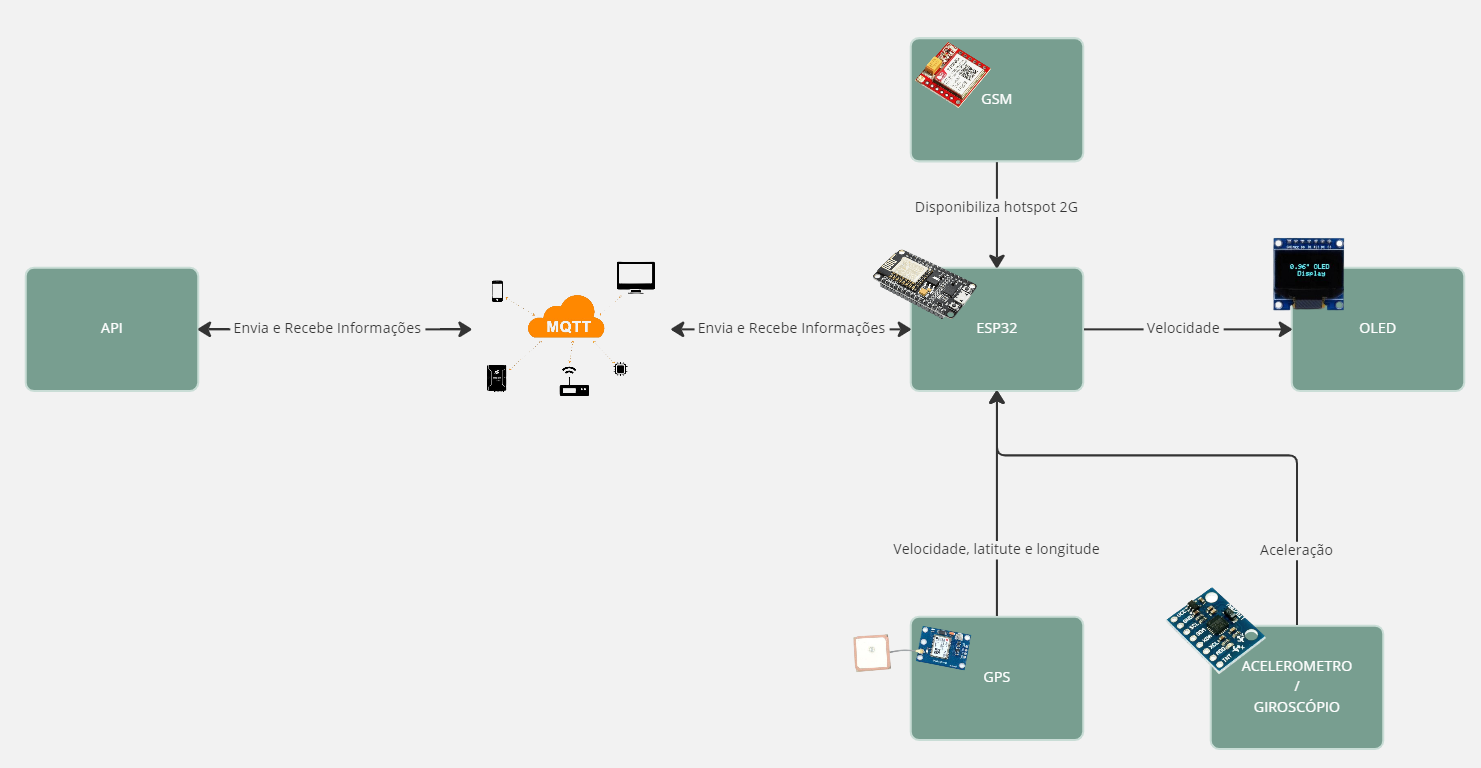
\includegraphics[width=15cm]{capitulos/Figuras/Diagrama_Hardware.png}
\caption{Diagrama geral do Projeto}
\label{fig:diagrama_hardware}
\end{figure} 

\section{Projeto mecânico}
\begin{figure}[!h]
\centering
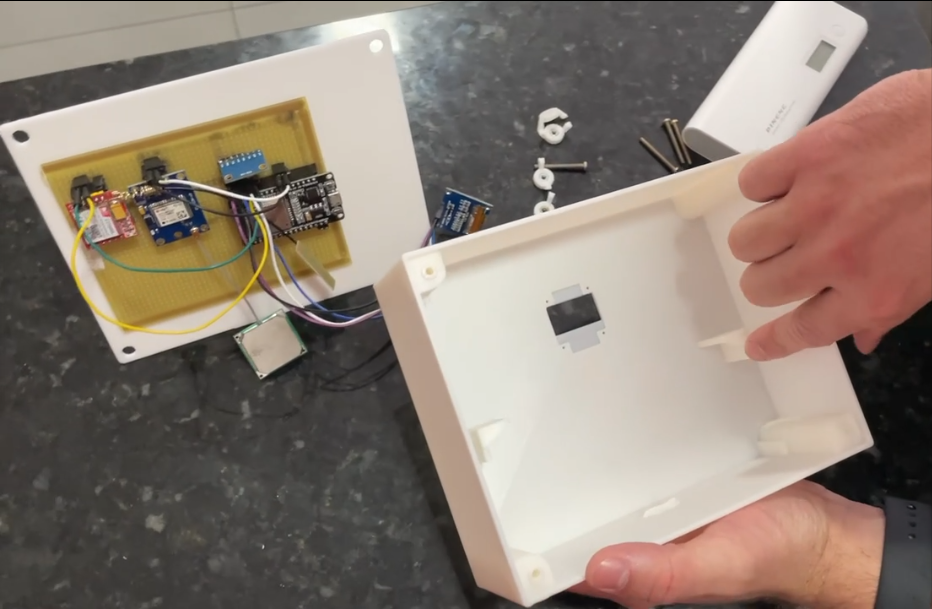
\includegraphics[width=15cm]{capitulos/Figuras/Mecanica.png}
\caption{Parte mecânica do projeto}
\label{fig:diagrama_hardware}
\end{figure}

Sobre a parte mecânica do projeto, esta foi feita quase que inteiramente por impressão 3D, usando PLA, como demonstrado nas Figuras \ref{fig:3d1} e \ref{fig:3d2}. Optou-se por utilizar o PLA devido ao seu baixo custo, mas acabamento e resistência satisfatórias. Assim, pode-se dividir o projeto em duas grandes partes mecânicas: a base do circuito com o suporte para fixação na bicicleta, e a tampa superior com um furo para posicionamento, exibição e fixação do display OLED.

Além disso, uma variável importante a se considerar na impressão 3D é o fluxo de polímero na ponteira. A base foi impressa com fluxo de 30 por cento, visando maior leveza e estabilidade na fixação do módulo. Já a tampa superior foi impressa com fluxo de 100 por cento, obtendo maior rigidez, robustez e opacidade, em detrimento da leveza.

\newpage

\begin{figure}[!h]
\centering
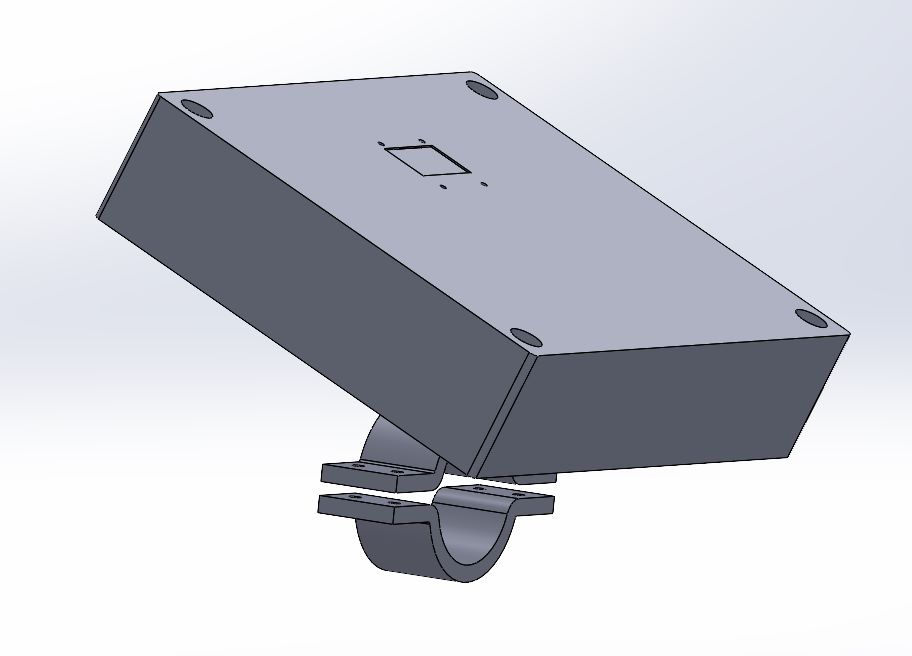
\includegraphics[width=13cm]{capitulos/Figuras/3d-1.jpg}
\caption{Visão isométrica do projeto 3D}
\label{fig:3d1}
\end{figure}

\begin{figure}[!h]
\centering
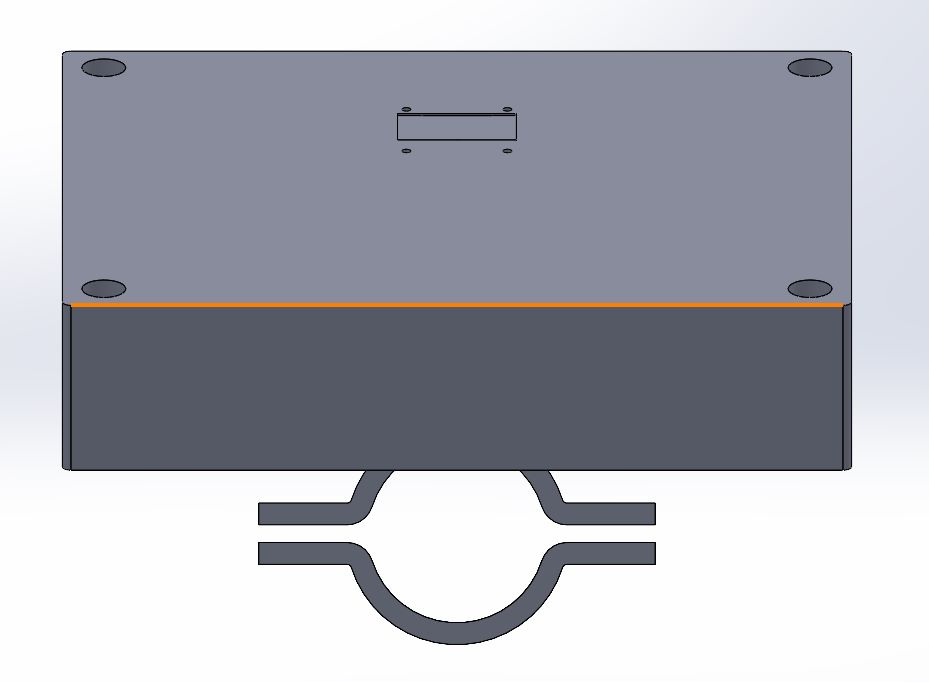
\includegraphics[width=13cm]{capitulos/Figuras/3d-2.jpg}
\caption{Visão frontal do projeto 3D}
\label{fig:3d2}
\end{figure}

\newpage
Em paralelo, foram impressas borboletas para envolver as porcas do projeto, a fim de auxiliar o usuário na fixação, desafixação e abertura do módulo quando necessário. Foram utilizados então parafusos e porcas avulsos, para fixação e ajuste do módulo.

Subsequentemente, foram realizados testes e experimentos a fim de validar a resistência do conjunto, com acelerações, movimentos bruscos e vibrações. Em todos os testes a montagem desempenhou muito bem, em nenhum momento deslizando ou abrindo demasiadamente.

\newpage
\section{Projeto de hardware}

Abaixo na Figura \ref{fig:diagrama_hardware} é possivel verificar um esquematico geral do projeto com o ESP32, GPS, OLED, acelerometro, GSM e a bateria de 7.4V.
\begin{figure}[!h]
\centering
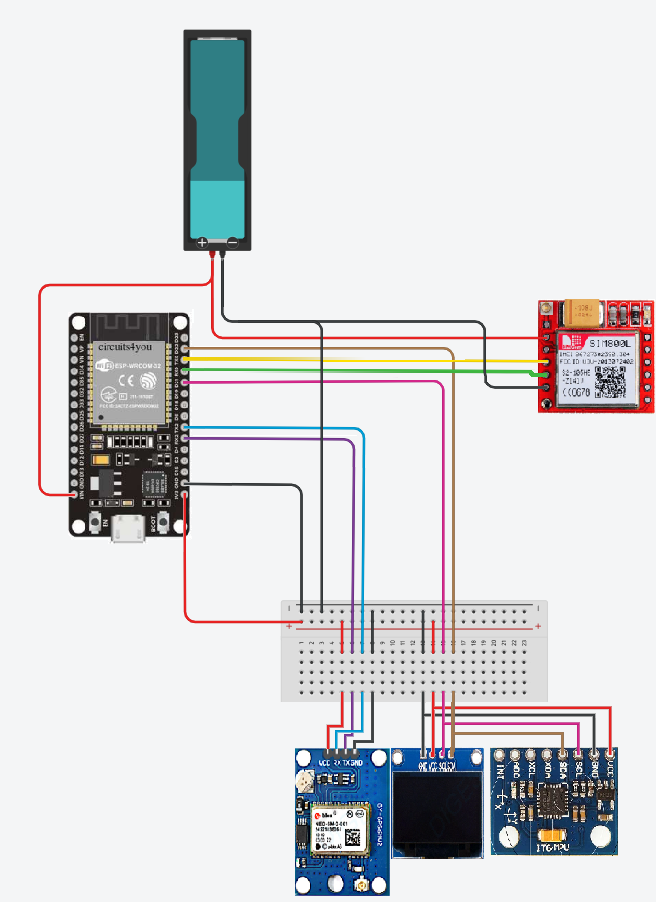
\includegraphics[width=15cm, height=20cm]{capitulos/Figuras/Circuito.png}
\caption{Circuito do projeto}
\label{fig:diagrama_hardware}
\end{figure}

\newpage
\section{Projeto de software}

O software do projeto é constituído em três partes, o software do microcontrolador, da API, e do aplicativo Android. Porém, para uma melhor explicação será apresentado o conjunto desses três componentes.

A comunicação Módulo-API é feita através de um broker MQTT da HiveMQ, para essa comunicação existem 4 tópicos. O ESP32 faz subscribe no tópico /bike/park (para receber o pedido de estacionar), e de forma contrária a API faz publish nesse tópico. O ESP32 também faz subscribe nos tópicos /bike/location (para enviar latitude, longitude e velocidade), /bike/warning (para avisar que a bicicleta saiu do lugar quando estacionada) e /bike/warning/state (para mostrar o estado atual da bicicleta, estacionada ou não), como demonstrado na Figura \ref{fig:mqtt_api_modulo}.

\begin{figure}[!h]
\centering
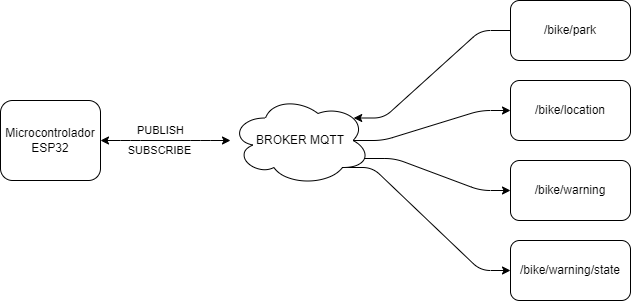
\includegraphics[width=15cm]{capitulos/Figuras/api-modulo.png}
\caption{Diagrama de comunicação ESP32-API via MQTT.}
\label{fig:mqtt_api_modulo}
\end{figure}

\newpage

A comunicação API-Aplicativo é feita de duas formas, uma via HTTP e outra via Firebase., demonstrados nas figuras \ref{fig:api_app_firebase} e \ref{fig:api_app_http}. Na comunicação via HTTP é feito um GET na rota /bike/lastLocation da API, assim retornando o último registro da latitude, longitude e velocidade da bicicleta.

\begin{figure}[!h]
\centering
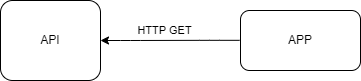
\includegraphics[width=10cm]{capitulos/Figuras/api-app.png}
\caption{Diagrama de comunicação API-Aplicativo via HTTP.}
\label{fig:api_app_firebase}
\end{figure}

\begin{figure}[!h]
\centering
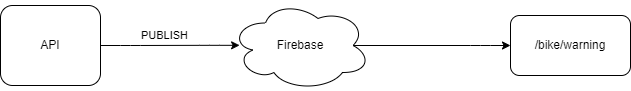
\includegraphics[width=15cm]{capitulos/Figuras/api-firebase.png}
\caption{Diagrama de comunicação API-Aplicativo via Firebase.}
\label{fig:api_app_http}
\end{figure}

Para o funcionamento do estacionamento da bicicleta, que é a ativação do modo de segurança da bicicleta, demonstrado na Figura \ref{fig:park-bike}. O fluxo começa com o usuário apertando o botão de estacionamento no aplicativo, que por sua vez envia um HTTP POST para a API, após isso é enviado um publish no /bike/park via MQTT e recebido no ESP32, após isso é desligado a tela OLED. Enquanto o modo estacionar estiver ligado o ESP32 irá monitorar o acelerômetro, e caso haja movimento (sendo um possível roubo) é enviado um MQTT publish para o tópico /bike/warning, que é recebido pela API e depois enviada para o aplicativo via Firebase. O fluxo termina com o usuário desativando o modo de estacionamento (caso não tenha sido ativado o \textit{warning}), que por sua vez envia um HTTP POST para a API, após isso é enviado um publish no /bike/park via MQTT e recebido no ESP32, após isso é ligado a tela OLED novamente, como demonstrado na Figura \ref{fig:unpark-bike}.

\begin{figure}[!h]
\centering
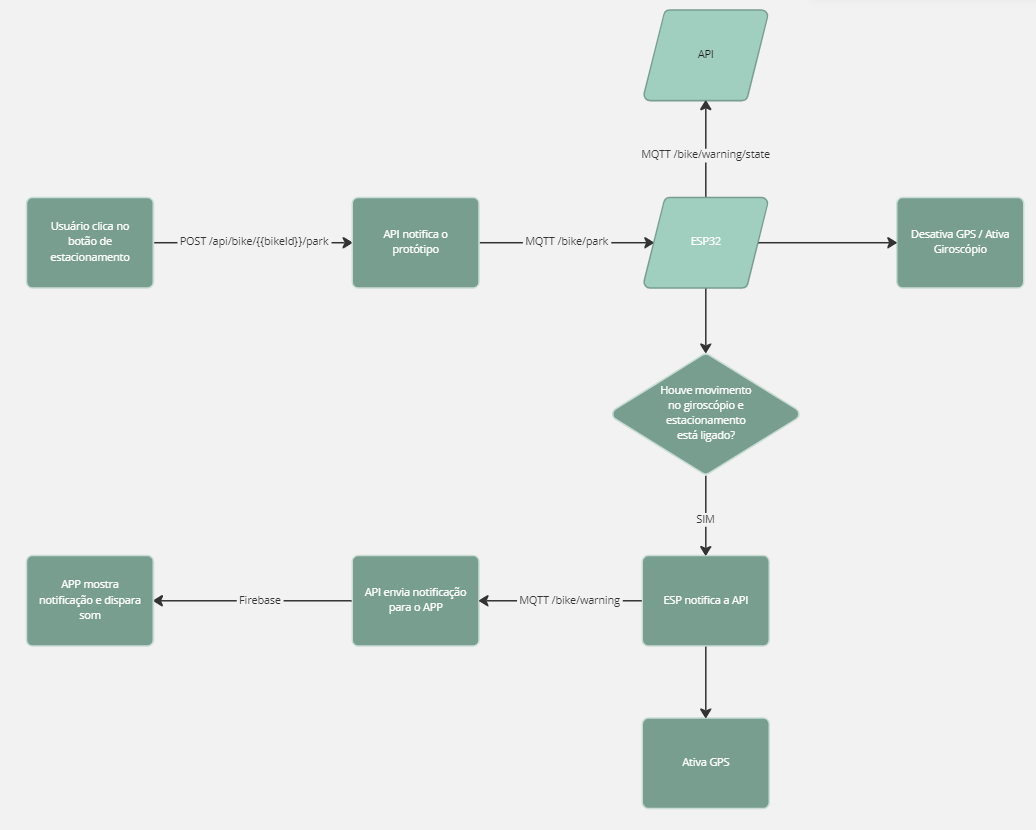
\includegraphics[width=15cm]{capitulos/Figuras/Software_Estacionar.png}
\caption{Software em modo estacionar.}
\label{fig:park-bike}
\end{figure}

\begin{figure}[!h]
\centering
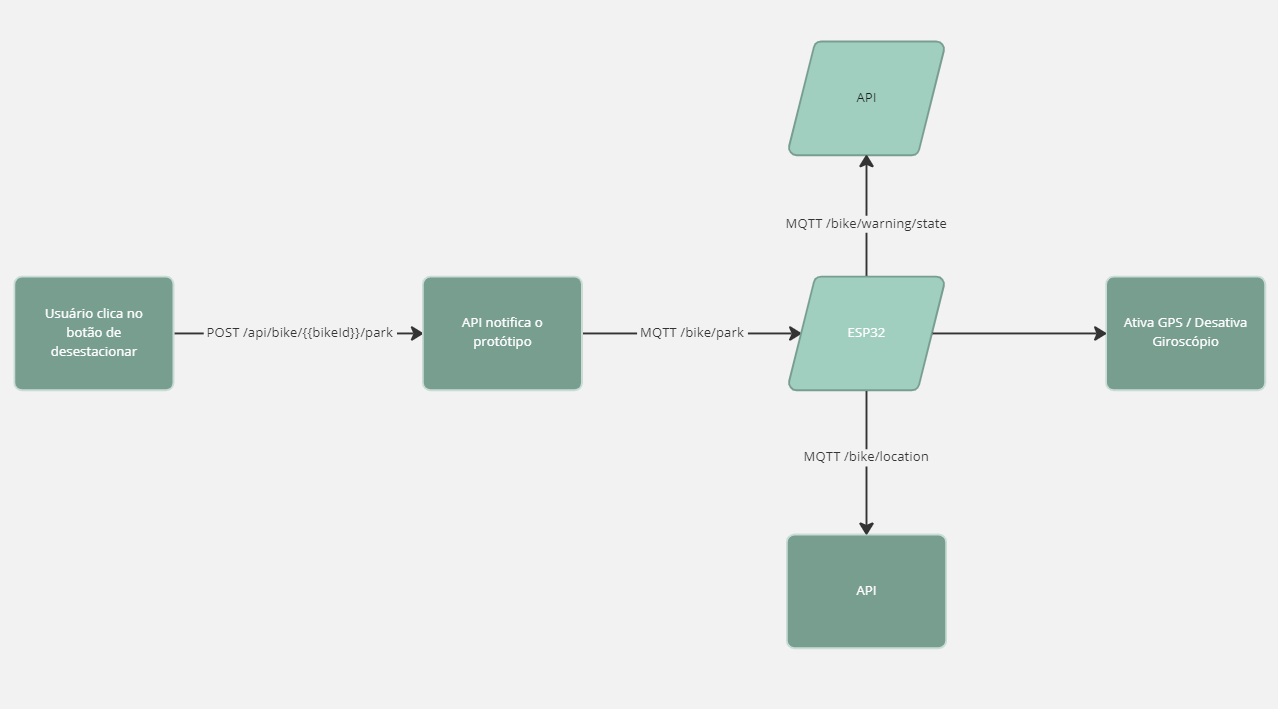
\includegraphics[width=15cm]{capitulos/Figuras/Software_Desestacionar.png}
\caption{Software em modo desestacionar.}
\label{fig:unpark-bike}
\end{figure}

\newpage
\section{Integração}
Por fim, a integração das fontes foi através de protocolos MQTT e HTTP. Por consequência, poucas mudanças basais no projeto ocorreram a partir de problemas de integração, as mudanças foram exclusivamente relacionadas com problemas de hardware, descritos com maior ênfase no tópico subsequente.